% Slide 2: the problem family. PEC unit square, dielectric disc, Gaussian current source.
\documentclass[border=8pt]{standalone}
% Shared preamble for the slide diagrams. Palette and ink colours match figures/make_figures.py.
\usepackage[T1]{fontenc}
\usepackage{dejavu}
\renewcommand{\familydefault}{\sfdefault}
\usepackage{amsmath,amssymb}
\usepackage{xcolor}
\usepackage{tikz}
\usetikzlibrary{arrows.meta,positioning,shapes.geometric,calc,fit,backgrounds,decorations.pathmorphing,patterns}

\definecolor{surface}{HTML}{FCFCFB}
\definecolor{ink}{HTML}{0B0B0B}
\definecolor{inktwo}{HTML}{52514E}
\definecolor{muted}{HTML}{898781}
\definecolor{gridc}{HTML}{E1E0D9}
\definecolor{axisc}{HTML}{C3C2B7}
\definecolor{cblue}{HTML}{2A78D6}
\definecolor{corange}{HTML}{EB6834}
\definecolor{cgreen}{HTML}{1BAF7A}
\definecolor{camber}{HTML}{EDA100}

\newcommand{\tg}[1]{{\scriptsize\color{inktwo}#1}}  % small secondary line inside a node

\pagecolor{surface}
\color{ink}

\tikzset{
  every node/.style={text=ink},
  % one box style; the argument is the role colour (blue learned, inktwo exact/fixed, corange verification, ...)
  box/.style={draw=#1, fill=#1!10, rounded corners=3pt, line width=0.9pt, align=center,
              inner xsep=6pt, inner ysep=5pt, minimum height=1.25cm, text width=2.75cm, font=\footnotesize},
  tag/.style={font=\scriptsize, text=inktwo, align=center},
  arr/.style={-{Stealth[length=5.5pt,width=4.5pt]}, line width=0.9pt, color=inktwo},
  darr/.style={arr, dashed},
}

\begin{document}
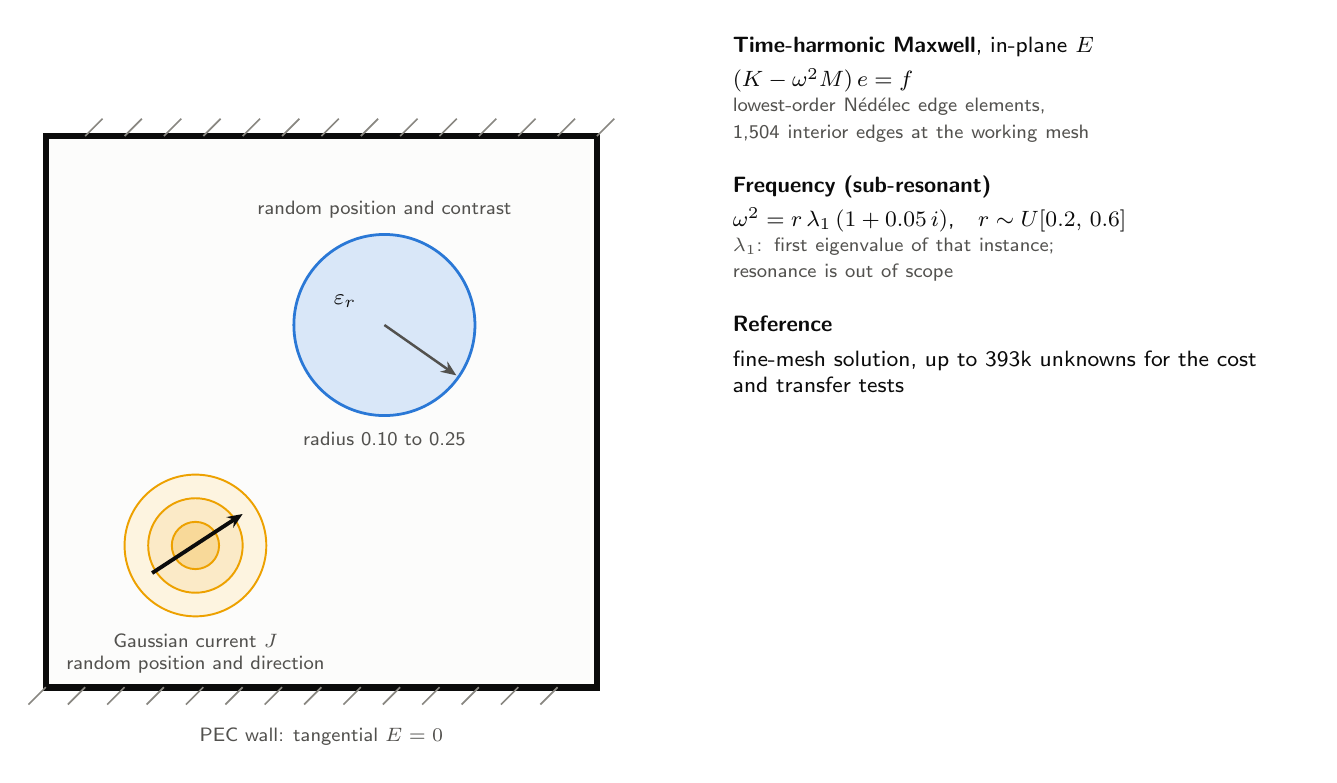
\begin{tikzpicture}[x=1cm,y=1cm]
  % cavity (unit square drawn at 7 cm)
  \def\L{7}
  \fill[surface] (0,0) rectangle (\L,\L);
  \draw[line width=2.4pt, color=ink] (0,0) rectangle (\L,\L);
  \foreach \i in {0,...,13}{
    \draw[color=muted, line width=0.6pt] (\i*0.5,0) -- ++(-0.22,-0.22);
    \draw[color=muted, line width=0.6pt] (\i*0.5+0.5,\L) -- ++(0.22,0.22);
  }
  \node[tag, anchor=north] at (\L/2,-0.4) {PEC wall: tangential $E=0$};

  % dielectric disc
  \def\cx{4.3} \def\cy{4.6} \def\rr{1.15}
  \draw[cblue, fill=cblue!18, line width=1pt] (\cx,\cy) circle (\rr);
  \node[font=\footnotesize] at (\cx-0.5,\cy+0.3) {$\varepsilon_r$};
  \draw[arr, shorten >=1pt] (\cx,\cy) -- ++(-35:\rr);
  \node[tag, anchor=north] at (\cx,\cy-\rr-0.08) {radius 0.10 to 0.25};
  \node[tag, anchor=south] at (\cx,\cy+\rr+0.08) {random position and contrast};

  % Gaussian current source
  \def\sx{1.9} \def\sy{1.8}
  \foreach \s/\o in {0.9/12, 0.6/22, 0.3/40}{
    \draw[camber, fill=camber!\o, line width=0.7pt] (\sx,\sy) circle (\s);
  }
  \draw[arr, color=ink, line width=1.4pt] (\sx-0.55,\sy-0.35) -- (\sx+0.6,\sy+0.4);
  \node[tag, anchor=north] at (\sx,\sy-1.0) {Gaussian current $J$\\random position and direction};

  % right-hand panel
  \node[anchor=west, align=left, font=\footnotesize, text width=7.2cm] at (8.6,\L-1.0) {%
    \textbf{Time-harmonic Maxwell}, in-plane $E$\\[3pt]
    $(K-\omega^2 M)\,e=f$\\[1pt]
    \tg{lowest-order N\'ed\'elec edge elements,\\1,504 interior edges at the working mesh}\\[10pt]
    \textbf{Frequency (sub-resonant)}\\[3pt]
    $\omega^2=r\,\lambda_1\,(1+0.05\,i)$,\quad $r\sim U[0.2,\,0.6]$\\[1pt]
    \tg{$\lambda_1$: first eigenvalue of that instance;\\resonance is out of scope}\\[10pt]
    \textbf{Reference}\\[3pt]
    fine-mesh solution, up to 393k unknowns for the cost and transfer tests};
\end{tikzpicture}
\end{document}
